\documentclass[12pt,onecolumn,a4paper]{article}
\usepackage{float}
\usepackage{epsfig,graphicx,subfigure,amsthm,amsmath}
\usepackage{color,xcolor}
\usepackage{xepersian}
\usepackage{graphicx}

\settextfont[Scale=1.2]{BZAR.TTF}
\setlatintextfont[Scale=1]{Times New Roman}


\begin{document}
\title{\lr{ENVISION OF PRODUCT} \\ پلتفرم اینترنتی فروش پوشاک}
\author{امیرمحمد فتاحی\\95000000 \and آرزو کاظمی دولت آبادی \\95194222 \and امیرحسین ایمانی\\96104087}
\date{\today}
\maketitle

\newpage
\tableofcontents
\newpage
\listoffigures
\newpage


\section{محدودیت محصول}
\subsection{تطبیق پذیری :}

سایت ما باید بتواند با شرایط مختلف تطبیق پذیرد و سازگار شود . برای مثال در صورت عدم موجودی سایت بلافاصله آپدیت شود و عدم موجودی را نمایش دهد . درصورت عدم وجود این موضوع مشتریان نارضایتی از محصول ما خواهند داشت . همچنین سایت باید با تکنولوژی های جدیدی که می آید به روز شود تا سهولت استفاده برای کاربران ایجاد کند .
\subsection{قابلیت اطمینان }
کاربران از ما انتظار دارند که 24 ساعته به آن ها سرویس بدهیم و در سرویس دهیمان وقفه به وجود نیاید . در واقع این ویژگی به انتظار کاربران به استفاده مداوم از پلتفرم ما باز میگردد . کاربران از ما انتظار دارند زمان در دسترس نبودن سایت به دلیل مسائل مختلف و فاصله ی بین این اتفاقات به حداقل خود برسد .

\subsection{مقیاس پذیری }
مقیاس پذیری باید در تکنولوژی ما باشد و بتوانیم با رشد غیر قابل پیش بینی تقاضا به هنگام شویم و غافلگیر نشویم . باید با استفاده از تجهیزات و ساختار ها و زیر بناهای قوی این مقیاس پذیری را در سایت خود ایجاد کنیم .

\subsection{امنیت}
همه ی فرآیند های اینترنتی امروزه به سطوح مشخصی از امنیت احتیاج دارند . یک نوع از امنیت به معنای حفاظت از مشتری می باشد و دیگری به حفاظت از شرکت می باشد . مهندسان سایت ما باید با وقت گذاری تاثیر عدم امنیت در سازمان را متوجه شوند و در صدد حفاظت از آن برآیند .  عمل امنیت باید در دو جبهه صورت گیرد : 1. حفاظت از اینترنت در برابر اسکمر ها 2. حفاظت از شرکت در مقابل دزدان

\subsection{قابلیت استفاده}
در دنیای امروزه قدرت در دست مشتریان قرار دارد . قابلیت استفاده یک محدودیت کالا است که به قدرت مشتری در استفاده از سایت ما باز میگردد . این ویژگی باید شامل
1.	حداکثر زمان بهینه ی پاسخگویی
2.	دسترسی 24 ساعته 7 روز در هفته
3.	قابلیت شخصی سازی نمایش سایت
4.	قابلیت فیلتر کردن اطلاعات
5.	قابلیت انتخاب محصولات
مهم ترین نکته ، در این نکته این است که چند کلیک طول میکشد تا به اطلاعات مورد نظر برسد و یا چرخه ی خود را تکمیل کند .

\subsection{قابلیت نگهداری}
هر چند ماه یکبار قابلیت های جدید به نرم افزار اضافه شود . یک نیازمندی نگهداری باید توسط صاحب سایت مشخص شود و طبق آن پیش رفت .


\section{نیازمندی های کارکردی}
\subsection{ثبت نام مشتری :}
1. ورود به سامانه\\
2. ثبت شماره همراه یا ایمیل \\
3. تکمیل مشخصات\\
4. دریافت پیامک تایید \\
5. تکمیل ثبت نام\\
\\
\\
\subsection{
ثبت نام صاحب فروشگاه  :
}
1. مراجعه حضوری\\
2. تکمیل مشخصات فروشگاه اعم از ساعت کاری و آدرس\\
3. عقد قرارداد با شرکت\\
4. ثبت در سامانه\\
5. دسترسی به سایت \\
6. امکان حذف و ویرایش و اضافه کردن محصولات به همراه مشخصاتشان\\
\\
\\

\subsection{
ثبت نام پیک موتوری  :
}
1. مراجعه حضوری\\
2. ثبت مشخصات خود\\
3. ثبت مشخصات وسیله نقلیه\\
4. ثبت در سامانه\\

\subsection{
ثبت درخواست توسط مشتری :
}
1.	ورود به سامانه\\
2.	دریافت لیست فروشگاه های نزدیک\\
3.	دریافت قیمت پیک\\
4.	انتخاب فروشگاه مد نظر\\
5.	مشاهده کالاهای موجود\\
6.	ایجاد سبد خرید شامل محصولات و تعداد آن ها\\
7.	انتقال به درگاه بانک\\
8.	پرداخت هزینه در سامانه از طریق درگاه بانک\\
9.	مشاهده موفقیت آمیز بودن تراکنش\\
10.	درصورت عدم موفیت تراکنش به گام شماره 7 باز میگردد \\
11.	دریافت محصول\\
12.	ارسال نظر و پیشنهاد به فروشگاه\\
13.	ارسال نظر و فروشگاه به پیک موتوری\\

\subsection{
ثبت درخواست ها توسط پیک :
}
1. تامین تلفن همراه به جهت ردیابی\\
2. قبول سفارش\\
3. دریافت اطلاعات خرید اعم از اطلاعات فروشگاه ، آدرس مقصد و لیست خرید \\
4. تحویل سفارش به مشتری\\

\subsection{
ثبت درخواست مرجوعی توسط مشتری :
}
1.	تماس با تیم پشتیبانی\\
2.	تحویل کالا به پیک\\

\subsection{
ثبت درخواست توسط صاحب فروشگاه :
}
1.	دریافت لیست خرید\\
2.	آماده سازی سبد خرید\\
3.	تحویل سفارش به پیک\\

\subsection{
ثبت درخواست توسط سیستم :
}
1.	نمایش لیست فروشگاه های نزدیک به مشتری و هزینه ارسال پیک\\
2.	بررسی لیست کالا های سفارش مشتری\\
3.	دریافت هزینه توسط درگاه بانک\\
4.	بررسی پیک های موتوری آنلاین\\
5.	انتخاب پیک موتوری\\
6.	نمایش اطلاعات خرید اعم از اطلاعات فروشگاه ، آدرس مقصد و لیست خرید\\
7.	درصورت رد درخواست توسط پیک مجددا جستجو انجام میگیرد\\
8.	دریافت و ذخیره امتیازات و نظرات\\
9.	نمایش امتیازات و نظرات\\

\newpage
\section{برد چشم انداز محصول\cite{3}(\lr{Product Vision Board})}
\begin{figure}[!h]
\centering{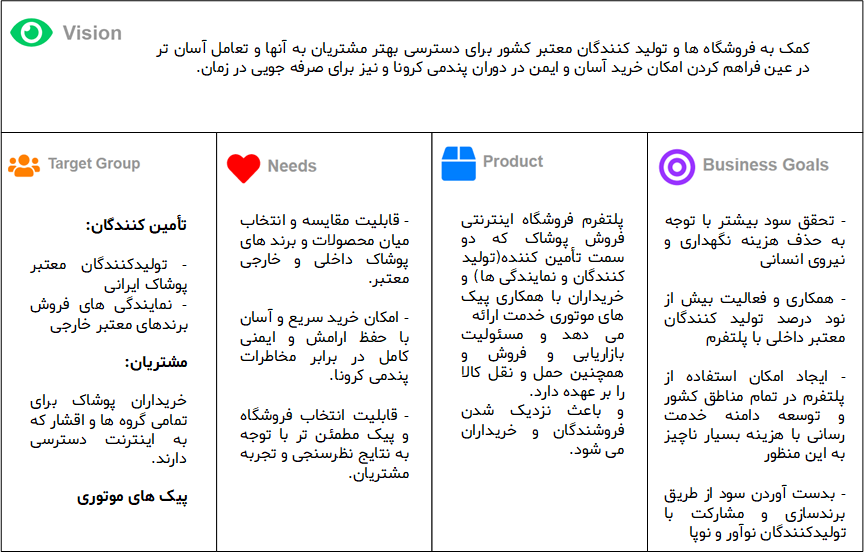
\includegraphics[width=14cm]{product_vision_board}}
\caption{\lr{product vision board}}\label{figpvb}
\end{figure}



\newpage

\section{داستان کاربری: } 


\subsection{مقدمه} 
داستان کاربر ابزاری است که در توسعه نرم افزار (چابک) به کار برده میشود تا خصوصیات یک نرم افزار را از دیدگاه یک کاربر نظاره گر باشد. داستان کاربر به شما میگوید که مخاطبان شما چه کسانی هستند، چه چیزی می خواهند و چرا؟
همان طور که بیان شد داستان کاربری یکی از راهکارهای دیدگاه چابک است. به این صورت که تمرکز از روی نیازها برداشته میشود و به تجربه کاربران و نظرات انها میپردازد.\\
\begin{figure}[h]

\includegraphics[scale=0.5]{cj}
\end{figure}

\subsection{ کاربران }
 1. مشتری 2. صاحب فروشگاه 3. پیک موتوری

\subsubsection{ مشتری }

به عنوان یک مشتری میخواهم پس سفارش خیلی سریع محصول به دستم برسد و در نزدیکی زمان تحویل  پیامکی جهت اینکه مطلع باشم که محصول به من خواهد رسید داشته باشم تا بتوانم حضور پیدا کنم.\\
\\
	

به عنوان یک مشتری میخواهم در سایت امکان فیلتر گذاری باشد (دخترونه و پسرونه یا از نظر قیمت یا سن) تا سریع تر بتوانم محصول خود را پیدا و انتخاب کنم.\\
\\


من به عنوان یک مشتری می‌خواهم که وقتی کالایی را در سایت برررسی میکنم دیتا ها   در لحظه باشد یعنی اگر کالا موجود نیست اطلاع رسانی شود تا محصول نا موجود را به اشتباه انتخاب نکنیم .\\
\\


به عنوان یک مشتری میخواهم نظرسنجی هاخیلی بررسی شود تا در مراحل بعدی مشکلی پیش نیایید و برطرف شود.\\
\\


به عنوان یک مشتری میخواهم فرایند خرید راحت و واضح باشد تا بتوانم با خیال اسوده خرید را انجام دهم.\\


به عنوان یک مشتری میخواهم اطلاعات جامع و کاملی از محصول اعم از جنس پارچه تا دچار مشکلاتی مانند پس فرستادن و نپذیرفتن از جانب شرکت نشود.\\
\\


به عنوان یک مشتری میخواهم کاربران سایت ما را راهنمایی کنند تا به مشکل برنخوریم.\\
\\

... چند هفته قبل اطلاع رسانی شود تا بتوانیم برنامه ریزی کنیم.\\
\\


به عنوان مشتری میخواهم در صورت داشتن مشکلی در کالا فروشگاه ان کالا را پس بگیرد تا حس رضایت و اعتماد بیشتر شود.\\
\\


به عنوان مشتری میخواهم در صورت رسیدن به یک عددی در خرید تخفیف ویژه به مشتریان بدهند تا وفاداری و حس خوب بیشتر شود به این سایت و....\\
\\
 
 تماس تلفنی و ... انجام شود تا بتوانم مشتری دائم شوم و فرایندها را یاد بگیرم و بیشتر خرید کنم.\\
\\

 برخورد مناسبی داشته باشند تا حس اعتماد بدست اورم و خرید بیشتری انجام دهم.\\
\\




\subsubsection{ صاحب فروشگاه  }

	  به عنوان یک صاحب فروشگاه میخواهم بعد از ارسال کالا یک نظر سنجی گذاشته شود تا سطح رضایت افراد را متوجه شویم چه از نظر به موقع بودن و چه از نظر کالای انتخابی\\
	  \\

 چه سمت و سویی است و بیشتر در چه رنج سنی و چه جنسیتی دارند.\\
\\


به عنوان یک صاحب فروشگاه گزارش می‌خواهم پیک موتوری سریع حاضر شوند و خیلی سری
ع مرسوله را به دست مشتری برسانند تا مشتریان به ما اعتماد کنند.\\
\\


 شود تا هم مشکلاتشان برطرف شود هم افراد دیگر هم با خواندن سوالات در صورت مشکل بتوانند انرا برطرف کنند.\\
\\


به عنوان یک صاحب فروشگاه گزارش می‌خواهم اطلاعات سریع اپدیت شود تا مشتریان به مشکل برنخورند و از خدمات راضی باشند.\\
\\


به عنوان یک صاحب فروشگاه گزارش می‌خواهم از نظر فنی سایت عالی باشد(سرعت و طراحی و...) تا مشتری لذت ببرد و حس رضایت داشته باشد و وفادار بماند.\\
\\


به عنوان یک صاحب فروشگاه می‌خواهم اطلاعات کالا را به خوبی بخوانند تا در صورت دریافت کالا مشکلی از لحاظ مثلا جنس پارچه و .... نداشته باشند.\\
\\


به عنوان یک صاحب فروشگاه می‌خواهم پول محصول را در کوتاه ترین زمان دریافت کنم تا بتوانم خریدهای اتی را انجام دهم.\\
\\










\subsubsection{پیک موتوری}

  من به عنوان یک پیک موتوری انتظار دارم که مشتریان ادرس را به صورت کامل و جامع ارسال کنند تا در جست و جوی مسیر مشکلی پیش نیاید.\\
  \\
  
  
من به عنوان یک پیک موتوری انتظار دارم شرکت تسهیلاتی را برای قائل شوند.\\
\\


به عنوان یک پیک موتوری می‌خواهم که بیمه شوم تا در صورت هر گونه اتفاق و خطری پیگیری شود.\\
\\


به عنوان یک پیک موتوری می‌خواهم رفتار خوبی از مشتریان داشته باشم تا انگیزه بگیرم برای ادامه کار.\\
\\


به عنوان یک پیک موتوری میخواهم در صورت راضی بودن امتیاز و نظر بدهند تا در صورت به دست اوردن امتیاز بالا پاداش دهند.\\
\\










\newpage
\begin{thebibliography}{99}
\bibitem{}
فایل توضیح پروژه
\bibitem{}
سایت سجایانگر
\bibitem{3}
\lr{www.romanpichler.com/blog/the-product-vision-board}
\bibitem{}
سایت کار و کسب


\end{thebibliography}




\end{document}



